%!TEX TS-program = lualatex
\RequirePackage{etex}
\documentclass[a4paper,oneside,12pt]{article}
\usepackage{fontspec}
   % http://tex.stackexchange.com/questions/132873/microtype-tracking-disables-small-caps-in-lualatex
   \defaultfontfeatures{SmallCapsFeatures={Renderer=Basic},}
   % Serif
   \setmainfont[%
      %Numbers=OldStyle,%
      Renderer=Basic%
      ]
      {Minion Pro}

   \setsansfont[%
      Renderer=Basic%
      ]      
      {TeX Gyre Heros}
      
\usepackage[protrusion=true, tracking=true]{microtype}
      
\usepackage{geometry}
   \geometry{
      marginparsep=1em,
      marginparwidth={0.2\linewidth},
      a4paper,
      left=0.28\linewidth,
      right=0.28\linewidth,
      bottom=0.3\linewidth
   }

\usepackage{tikz}
\usepackage{parskip}
\usepackage[scale=2.0]{ccicons}
\usepackage{xcolor}
   % Use the UOW colour pallet
   \definecolor{UOWblack}{RGB}{0, 0, 0}
   \definecolor{UOWgold}{RGB}{253, 184, 19}
   \definecolor{UOWdarkblue}{RGB}{0, 83, 154}
   \definecolor{UOWred}{RGB}{238, 64, 52}
   \definecolor{UOWblue}{RGB}{0, 149, 214}
   \definecolor{UOWdarkgreen}{RGB}{0, 146, 94}
   \definecolor{UOWlimegreen}{RGB}{183, 198, 38}
   \definecolor{UOWorange}{RGB}{243, 121, 32}
   \definecolor{UOWdarkred}{RGB}{195, 18, 48}
   \definecolor{UOWpink}{RGB}{238 ,0, 139}
   \definecolor{UOWpurple}{RGB}{74, 47, 142}
   \definecolor{UOWgrey}{RGB}{69, 85, 95}

\usepackage{titlesec}
    \titleformat{\section}
        {\color{UOWblue}\normalfont\large\sffamily}
        {\color{UOWblue}\thesection}{1em}{}

\usepackage{lipsum}
\usepackage{multicol}
\usepackage{marginfix}
\usepackage{marginnote}
   \reversemarginpar

\usepackage{pdfpages}
\usepackage[colorlinks=true, allcolors=UOWdarkblue]{hyperref}

\newenvironment{absolutelynopagebreak}
  {\par\nobreak\vfil\penalty0\vfilneg
   \vtop\bgroup}
  {\par\xdef\tpd{\the\prevdepth}\egroup
   \prevdepth=\tpd}

\setlength{\fboxsep}{0pt}%
\setlength{\fboxrule}{1pt}%
\newcommand{\key}[1]{\texttt{\color{UOWorange}#1}} 
\newcommand{\val}[1]{\texttt{\color{UOWblue}#1}} 
\newcommand{\command}[1]{\texttt{\color{UOWdarkgreen}#1}} 

\title{\textsf{The UOW Beamer Theme}}
\author{Thomas M. Griffiths}
\date{Released \today, Version 1.0}

\begin{document}

\maketitle

\section{About}
This theme ports the UOW Power Point templates over to Beamer, a \LaTeX class for presentations. The template has been set up so that the layout for the entire presentation is selected and the slides are formatted as appropriate, individual slides cannot be themed at this stage. See section \ref{sec:options} for examples. Each layout can be coloured with the UOW Branding colours, which are available also for the user to use as colours for objects in their presentation. The entire theme consists of eight files in total: five files, a demo and two logos. 
\begin{multicols}{2}
\begin{itemize}
   \item \texttt{\colorbox{UOWgrey!20}{beamerthemeuow.sty}},
   \item \texttt{\colorbox{UOWgrey!20}{beamerouterthemeuow.sty}},
   \item \texttt{\colorbox{UOWgrey!20}{beamerinnerthemeuow.sty}},
   \item \texttt{\colorbox{UOWgrey!20}{beamercolorthemeuow.sty}},
   \item \texttt{\colorbox{UOWgrey!20}{beamerfontthemeuow.sty}},
   \item \texttt{\colorbox{UOWgrey!20}{demo.tex}},
   \item \texttt{\colorbox{UOWgrey!20}{UOW\_mono.pdf}} and
   \item \texttt{\colorbox{UOWgrey!20}{UOW\_mono\_inverted.pdf}}.
\end{itemize}
\end{multicols}

The author maintains the code for this Beamer theme on \href{https://github.com/tmgriffiths/UOW_Beamer}{GitHub.} If you have any comments or suggestions please get in touch there.

\section{Usage}
To use the theme in your presentation simply place the files in the working directory of your latex document. In your document load the theme via:\\

\command{\textbackslash{}documentclass\{beamer\}}\\
\command{\textbackslash{}usetheme[\key{key}=\val{value}, \key{key}=\val{value}]\{uow\}}\\

Note, that the \command{\key{key}=\val{value}} entries are optional. For an explanation of each \key{key} and \val{value} see section \ref{sec:options}. The defaults values for the theme are \key{themecolor}=\val{blue}, \key{layout}=\val{standard} and \key{framenumbering}=\val{none}; these are what will be loaded if no options are specified with \command{\textbackslash{}usetheme\{uow\}}. 

All the standard options for a beamer class; aspect ratio, fontsize etc. are still available. To get the two slide ratios offered by the UOW Power Point theme use the following options for the \emph{document class}: \key{aspectratio}=\val{43} for a 4:3 aspect ratio, and \key{aspectratio}=\val{169} for a 16:9 aspect ratio. For a example presentation compile \texttt{demo.tex}.

This theme is currently \emph{not} distributed via CTAN. It is only available via download from UOW, or you may download, clone or fork the repository on \href{https://github.com/tmgriffiths/UOW_Beamer}{Github}\footnote{\url{https://github.com/tmgriffiths/UOW_Beamer}}. Distribution by CTAN may be implemented in the future.

\section{Package Options}\label{sec:options}
\subsubsection*{\key{layout}}%
In the Microsoft Power point implementation there are three main frame styles. One with solid colour for the background of the slide and a thin white polygon at the base containing the UOW brandmark. A style that is the inverse of this, a white background with coloured polygon. And a third eco style with a white background and an just the outline of the polygon at the base of the slide.

While individual slides can't be themed at this stage there are eight layouts included in this theme. These eight options should encompass most sensible arrangements of slides, these options are shown below with the default blue colour.

If your presentation won't have a title page you can turn the different layout for the first page with the \key{titlepage}=\val{false} or \val{none}. The default is \val{true}.

\subsubsection*{\val{standard} default}% \hfill \textbf{default} \\[0.5em]
\fbox{
\includegraphics[width=0.5\textwidth]{titleframe_standard.png}}
\fbox{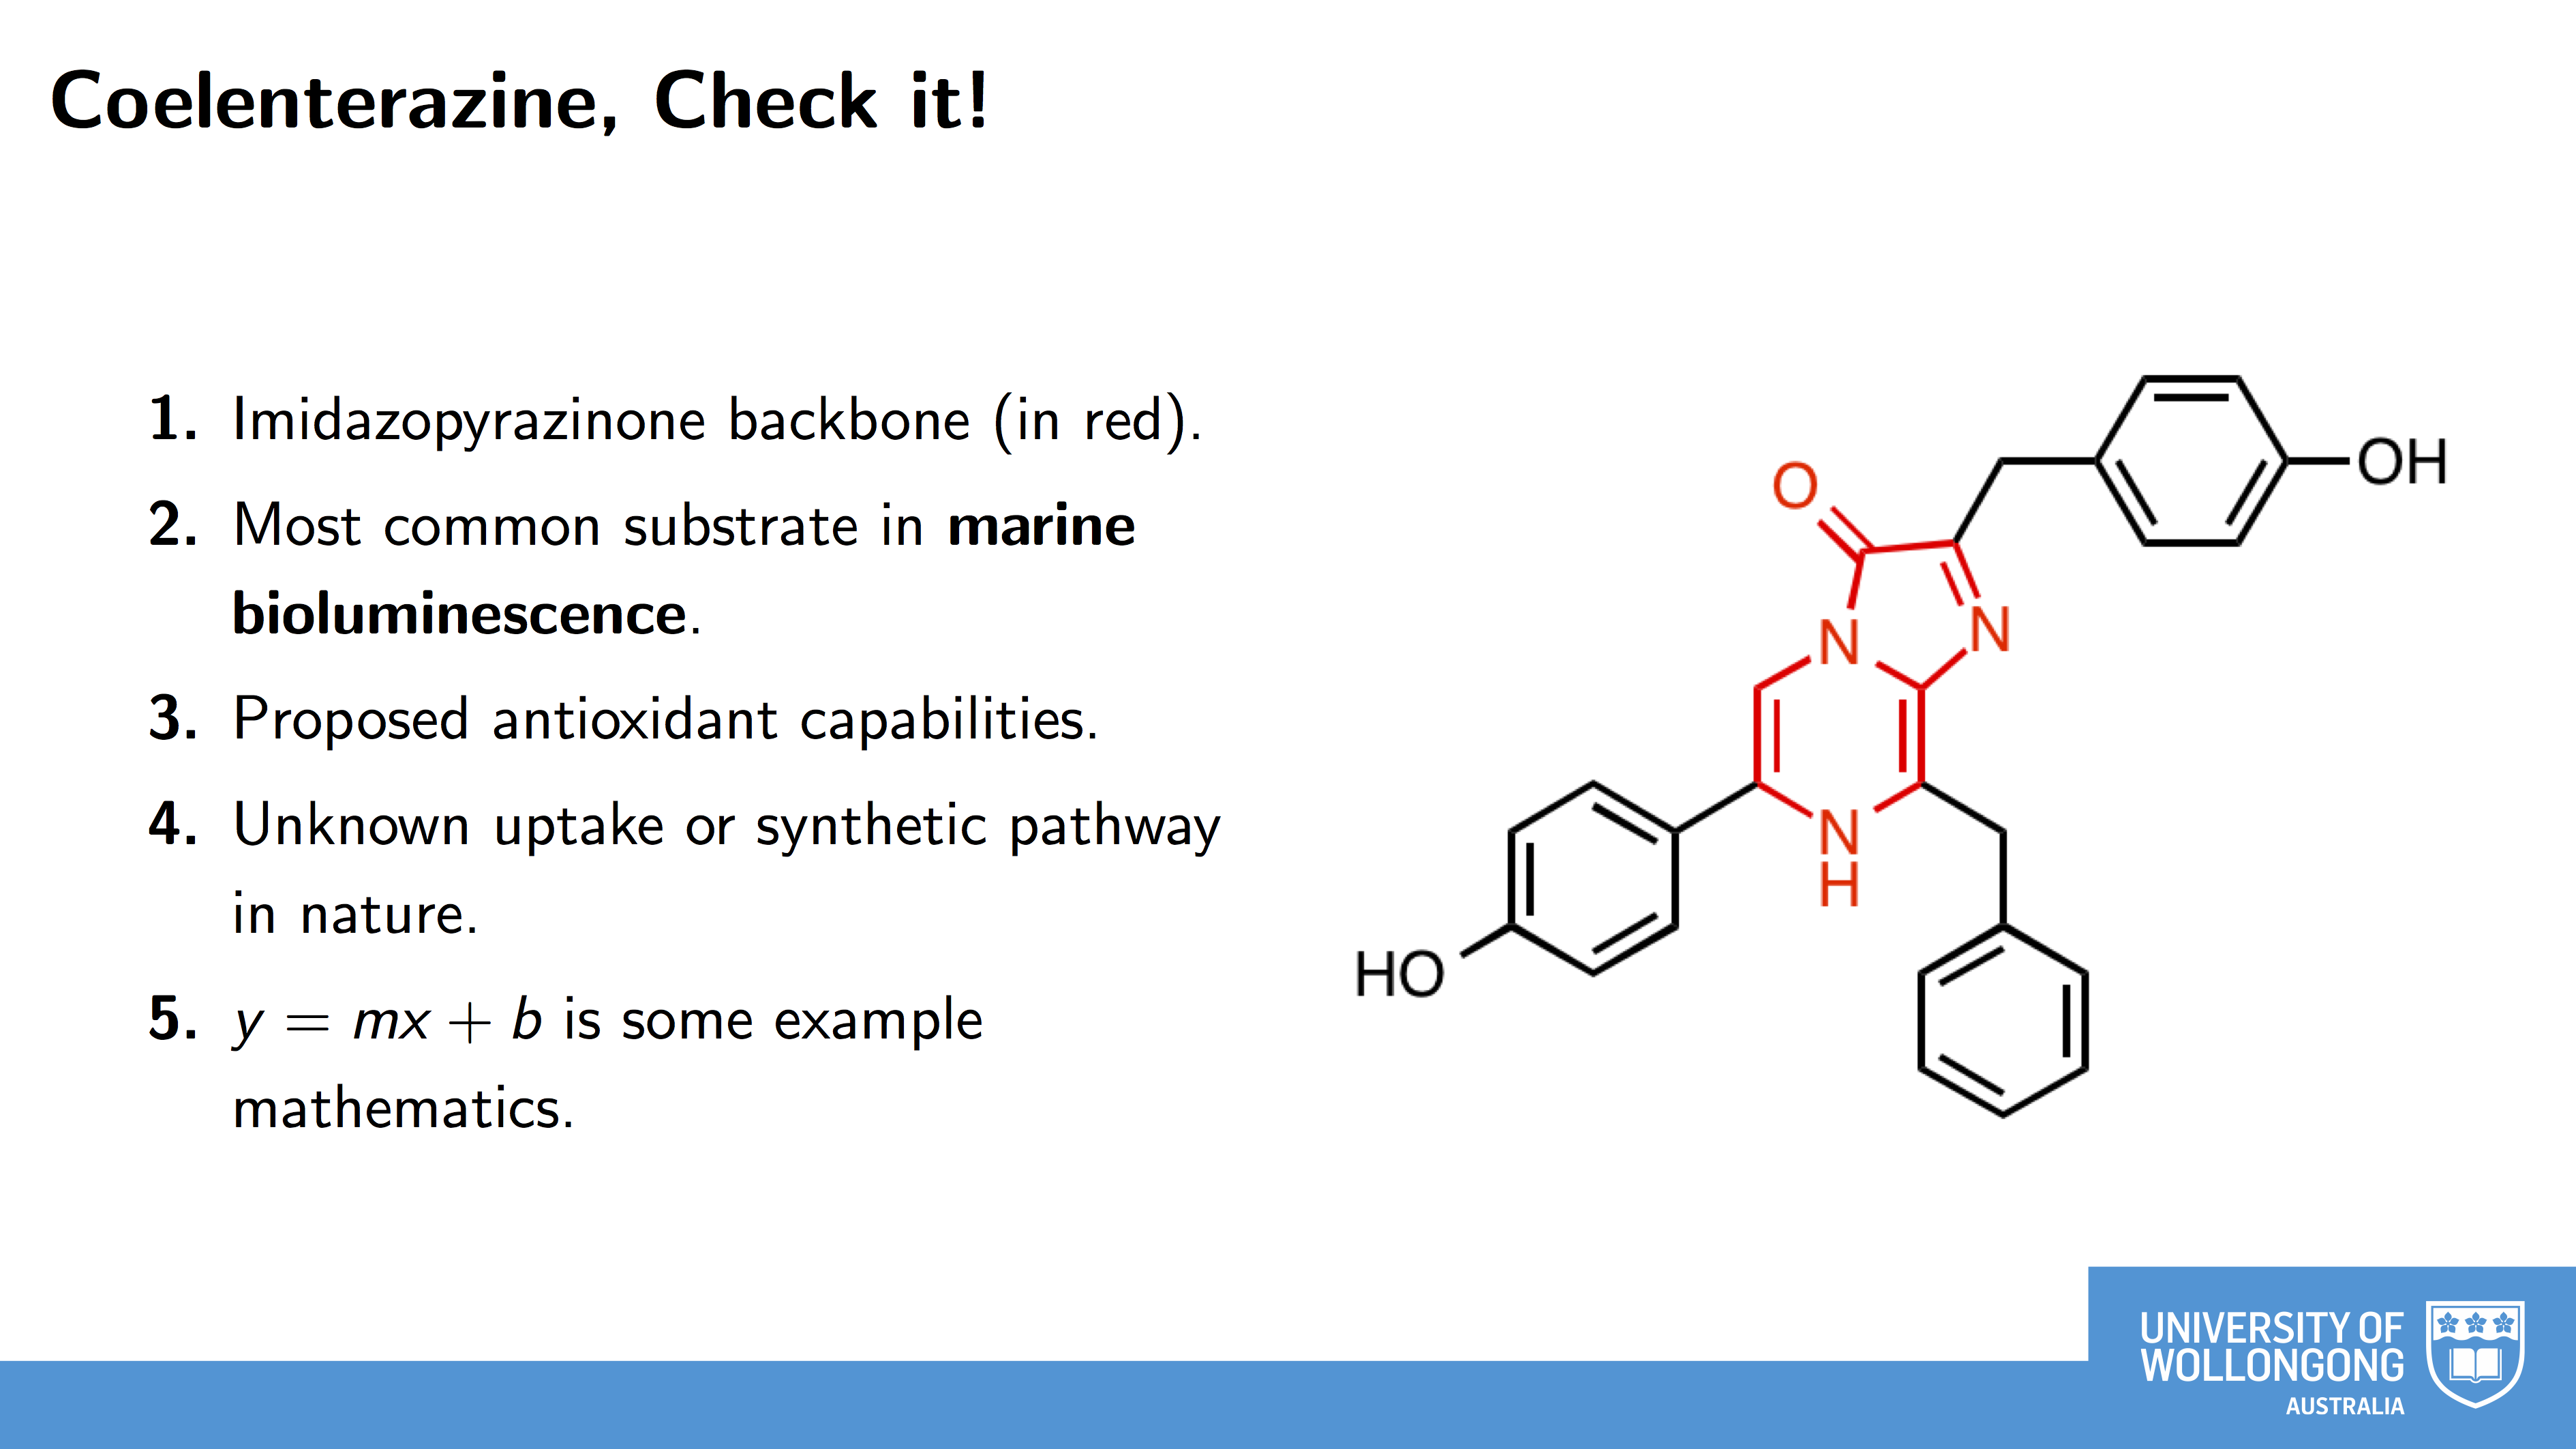
\includegraphics[width=0.5\textwidth]{contentframe_standard.png}}\par

\subsubsection*{\val{minimaltitle}}% \\[0.5em]
\fbox{
\includegraphics[width=0.5\textwidth]{titleframe_minimal.png}}
\fbox{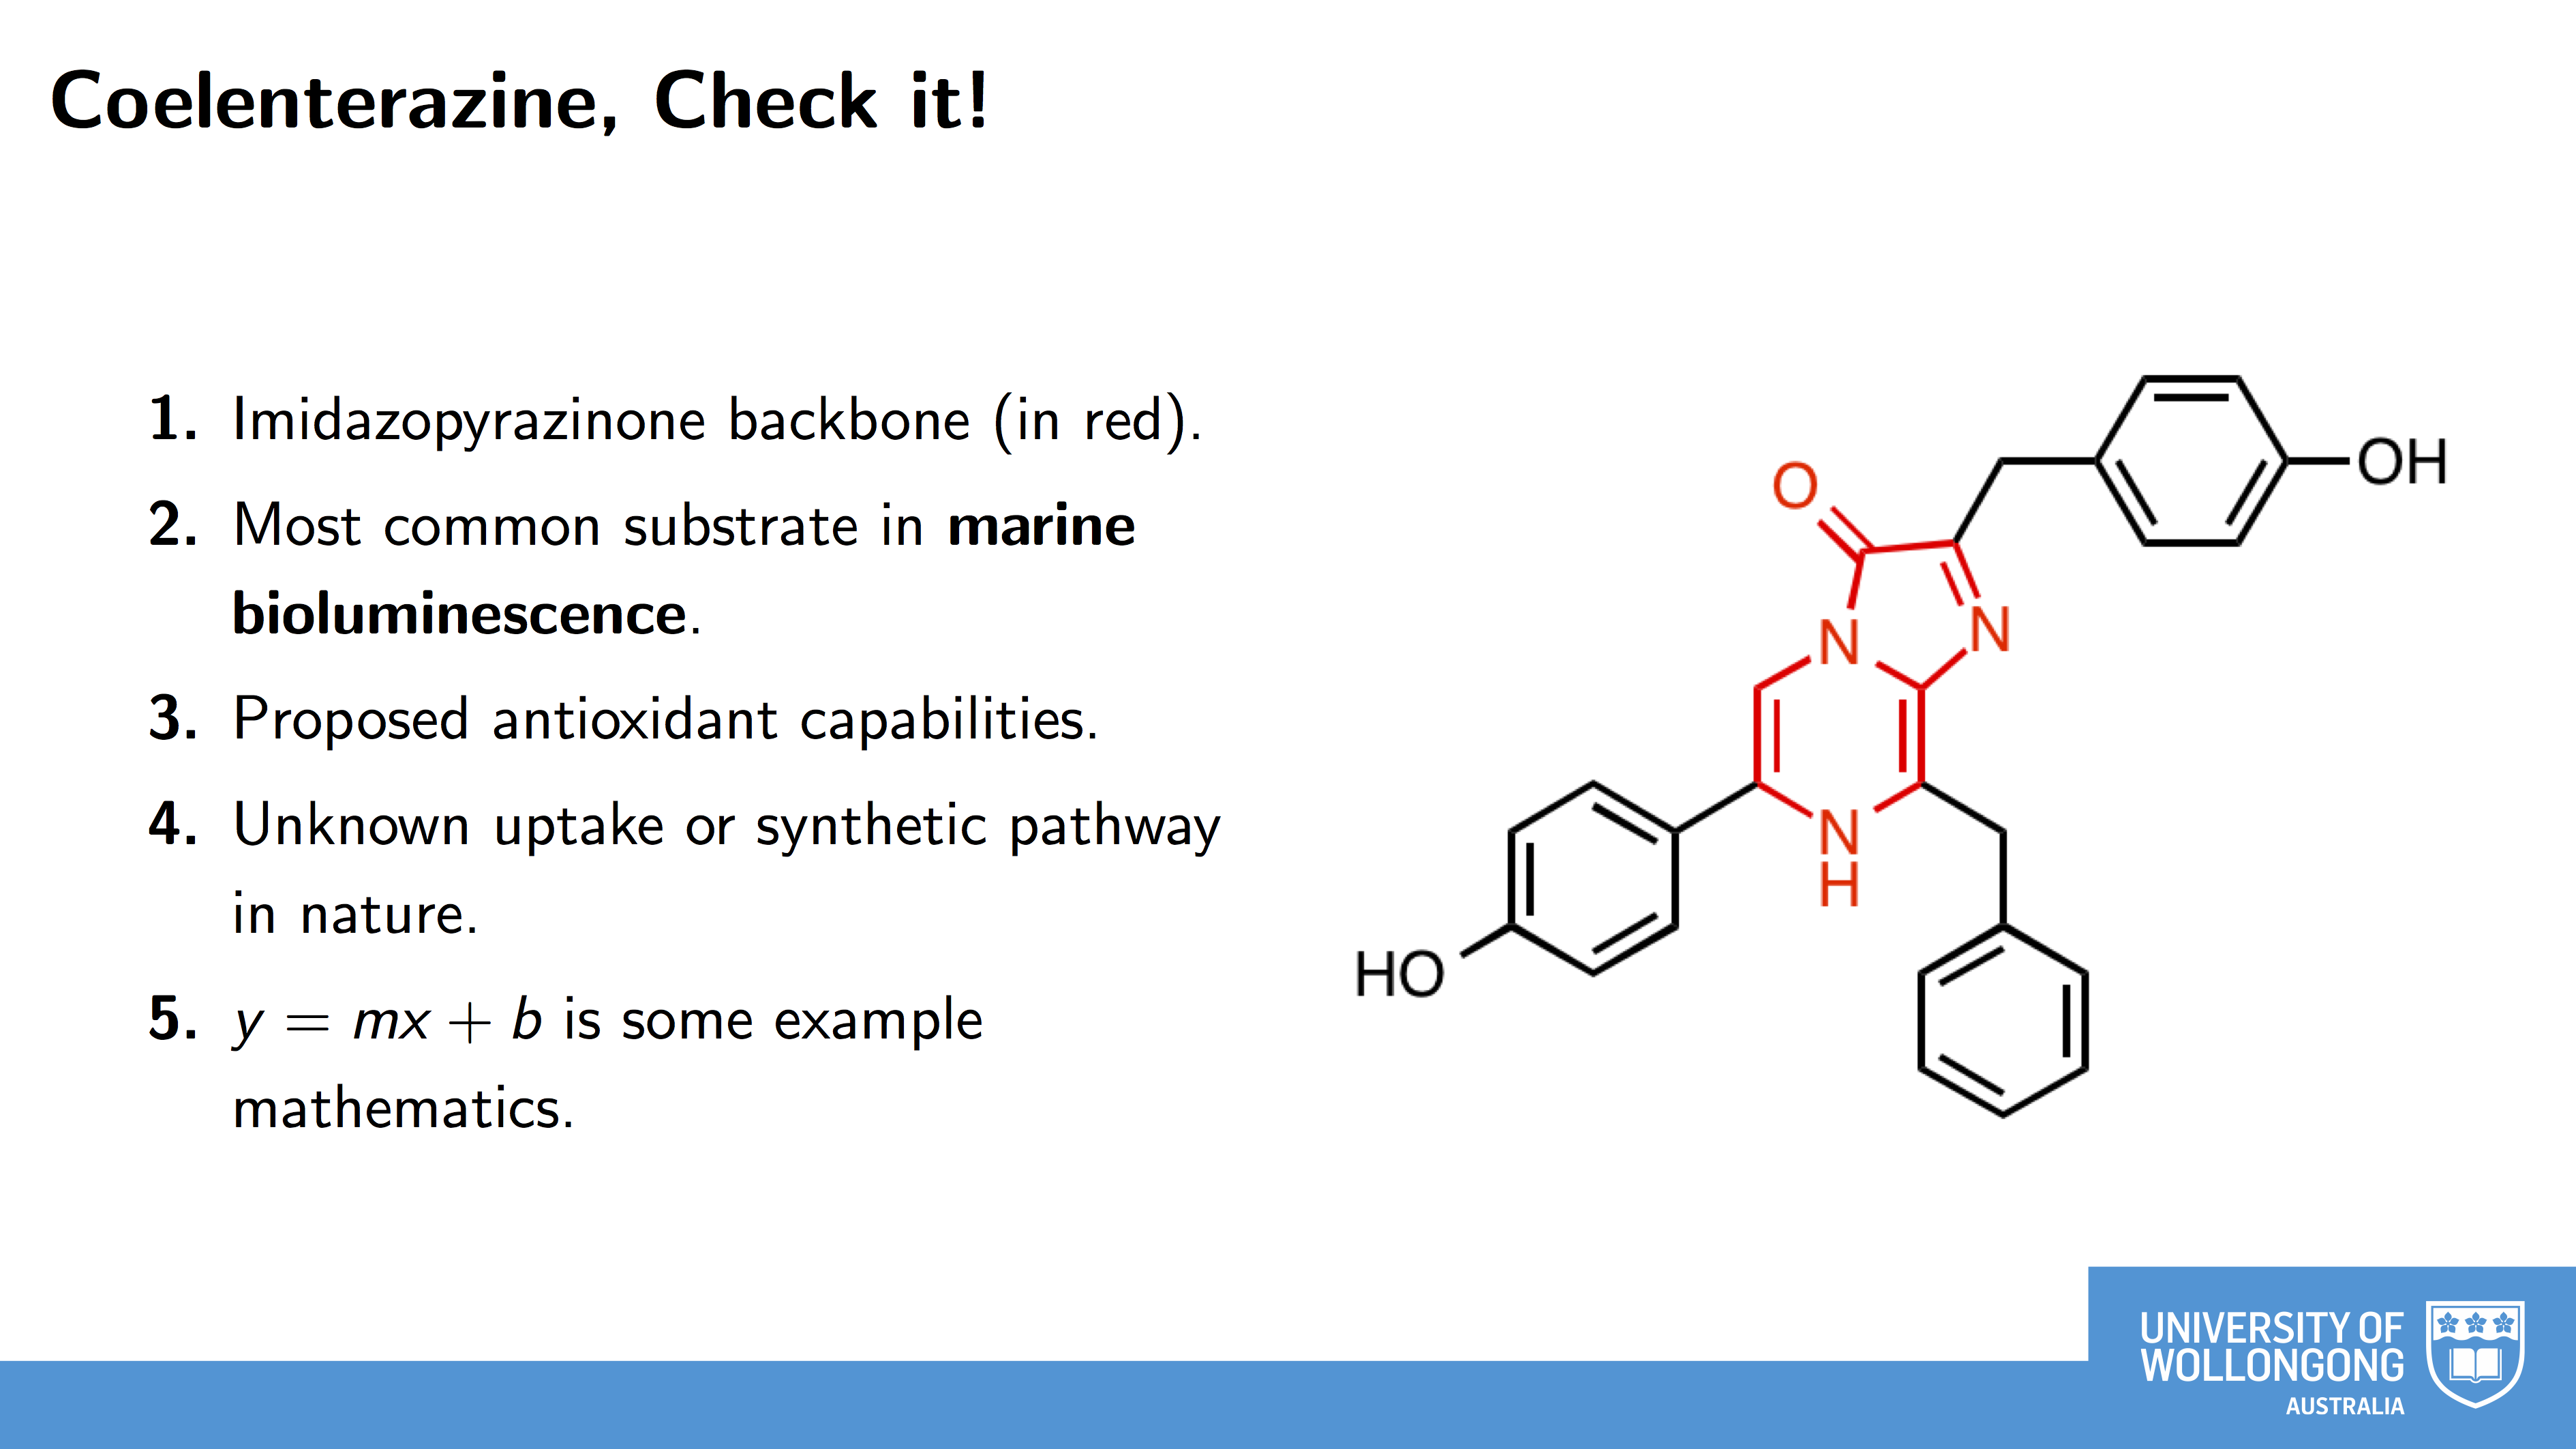
\includegraphics[width=0.5\textwidth]{contentframe_standard.png}}\par

\subsubsection*{\val{minimal}}% \\[0.5em]
\fbox{
\includegraphics[width=0.5\textwidth]{titleframe_minimal.png}}
\fbox{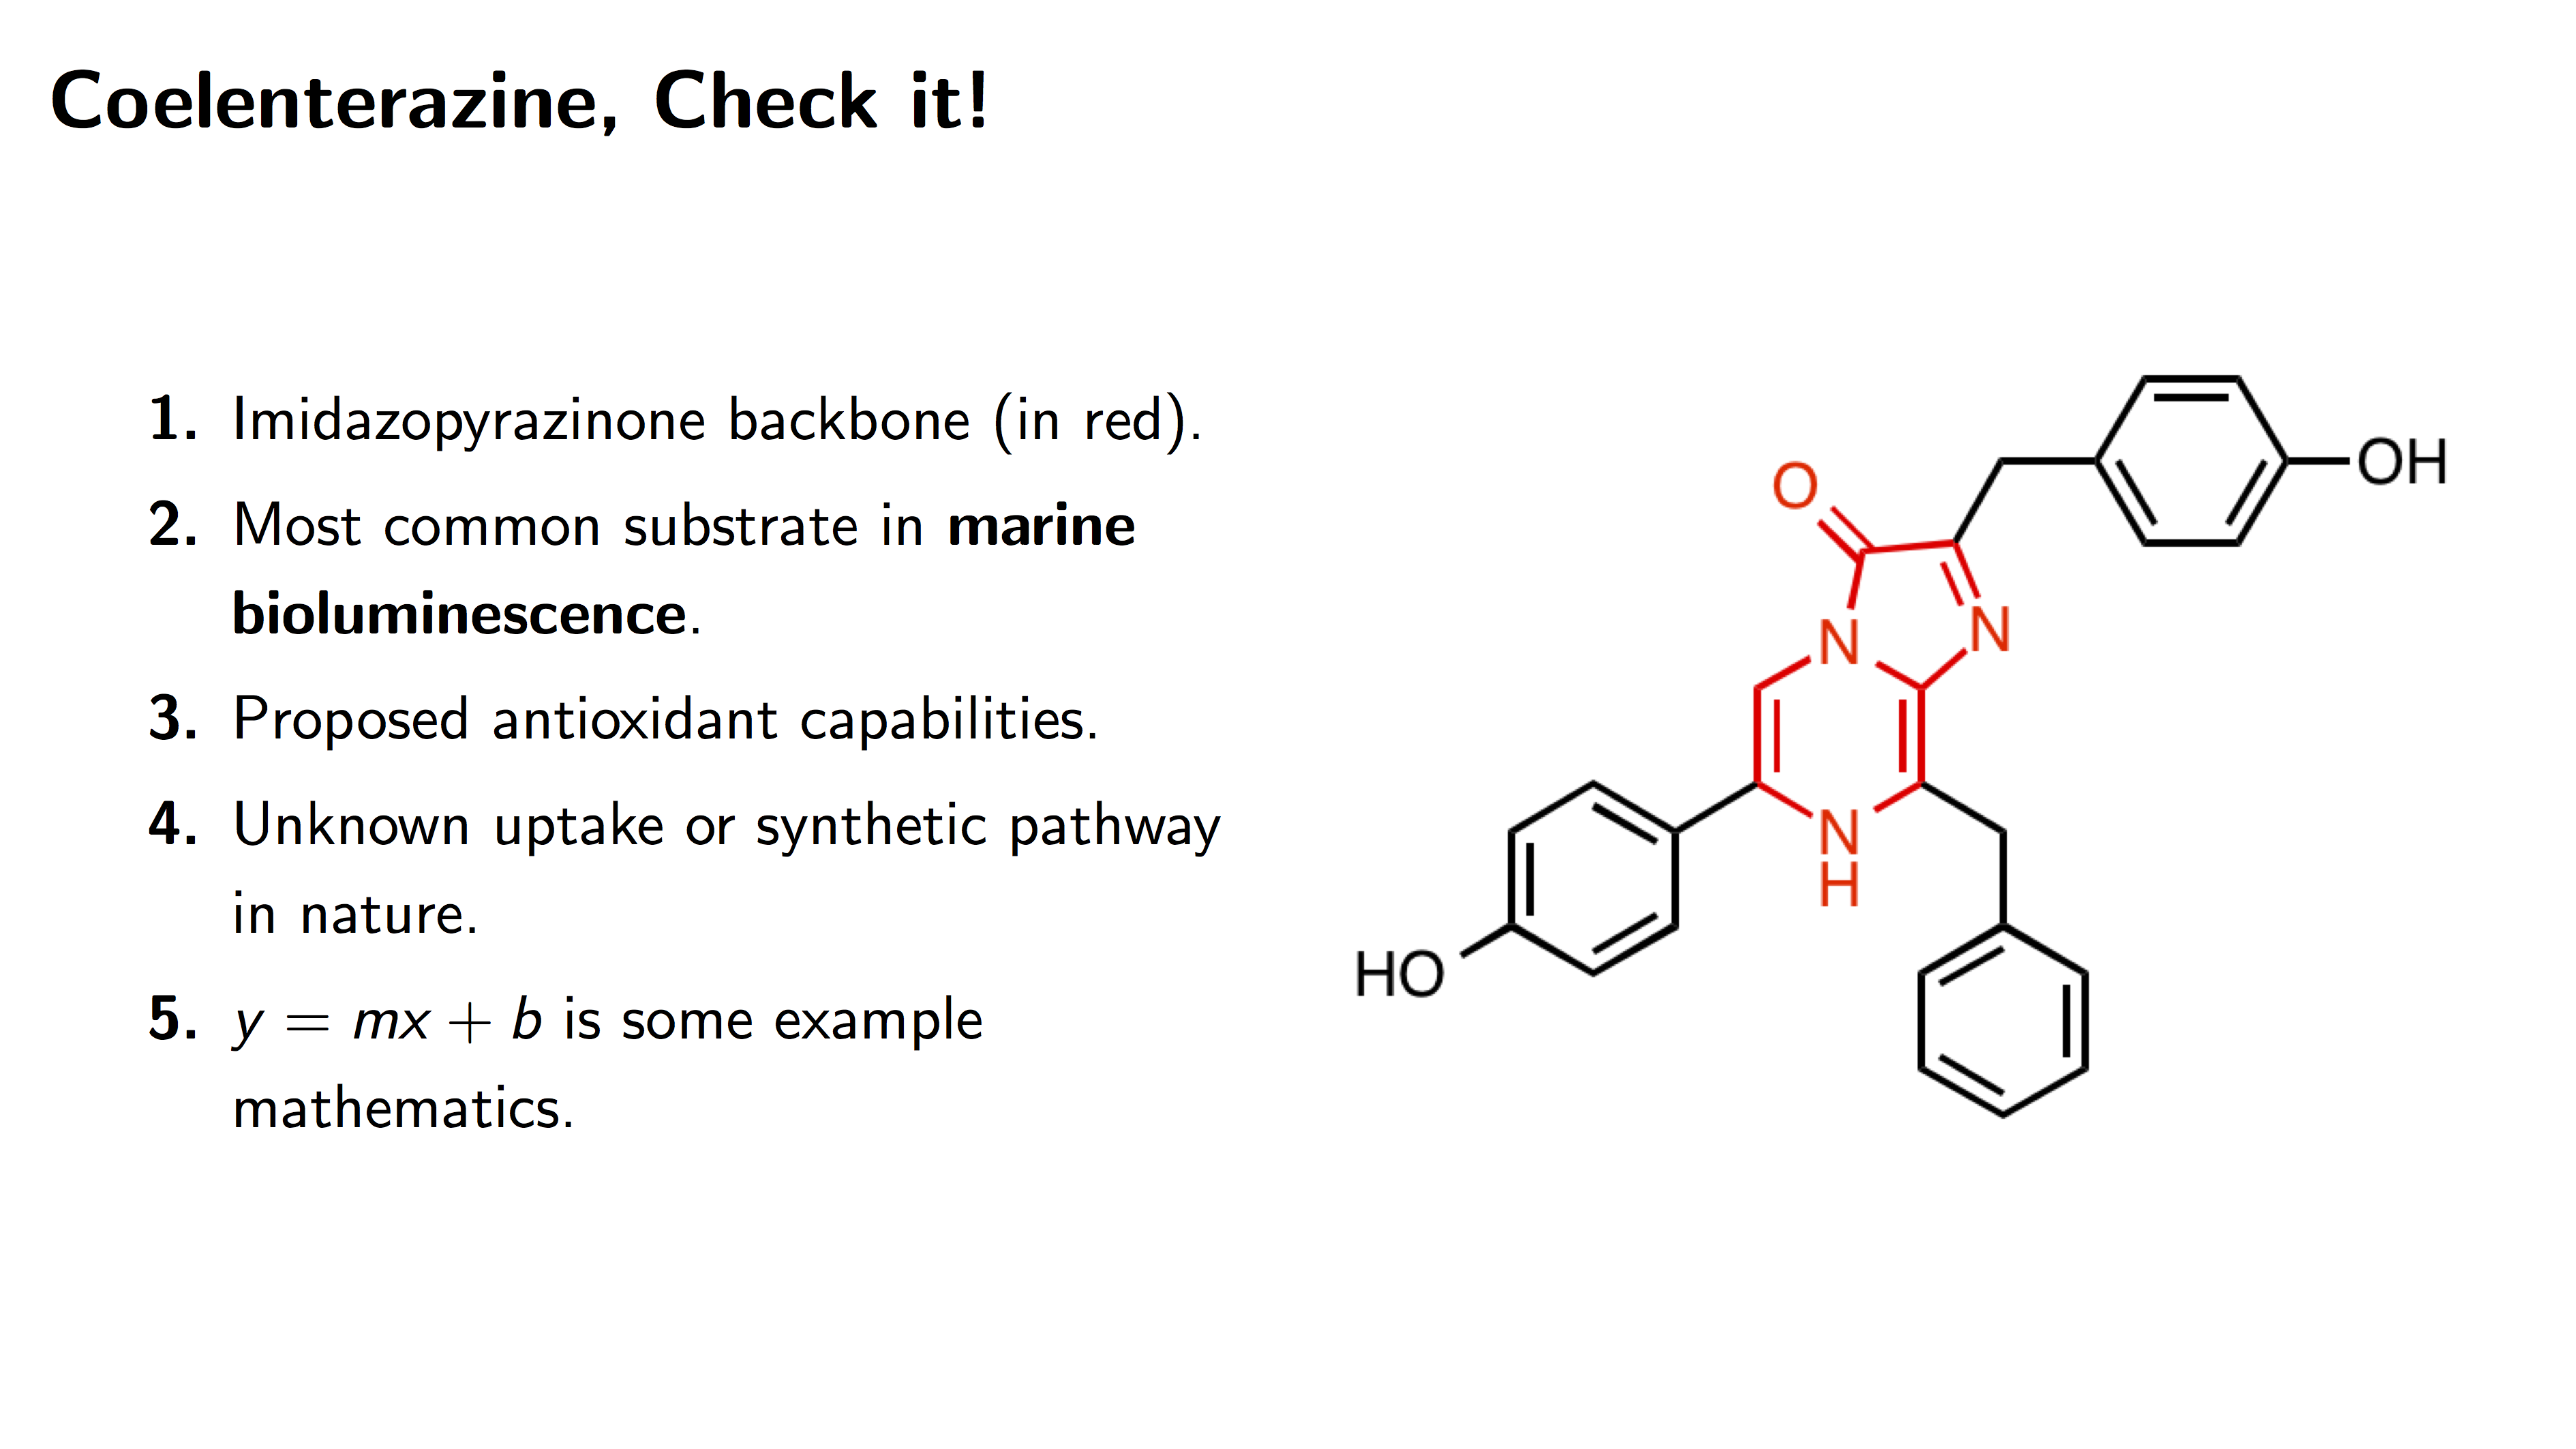
\includegraphics[width=0.5\textwidth]{contentframe_plain.png}}\par

\subsubsection*{\val{bold}}% \\[0.5em]
\fbox{
\includegraphics[width=0.5\textwidth]{titleframe_standard.png}}
\fbox{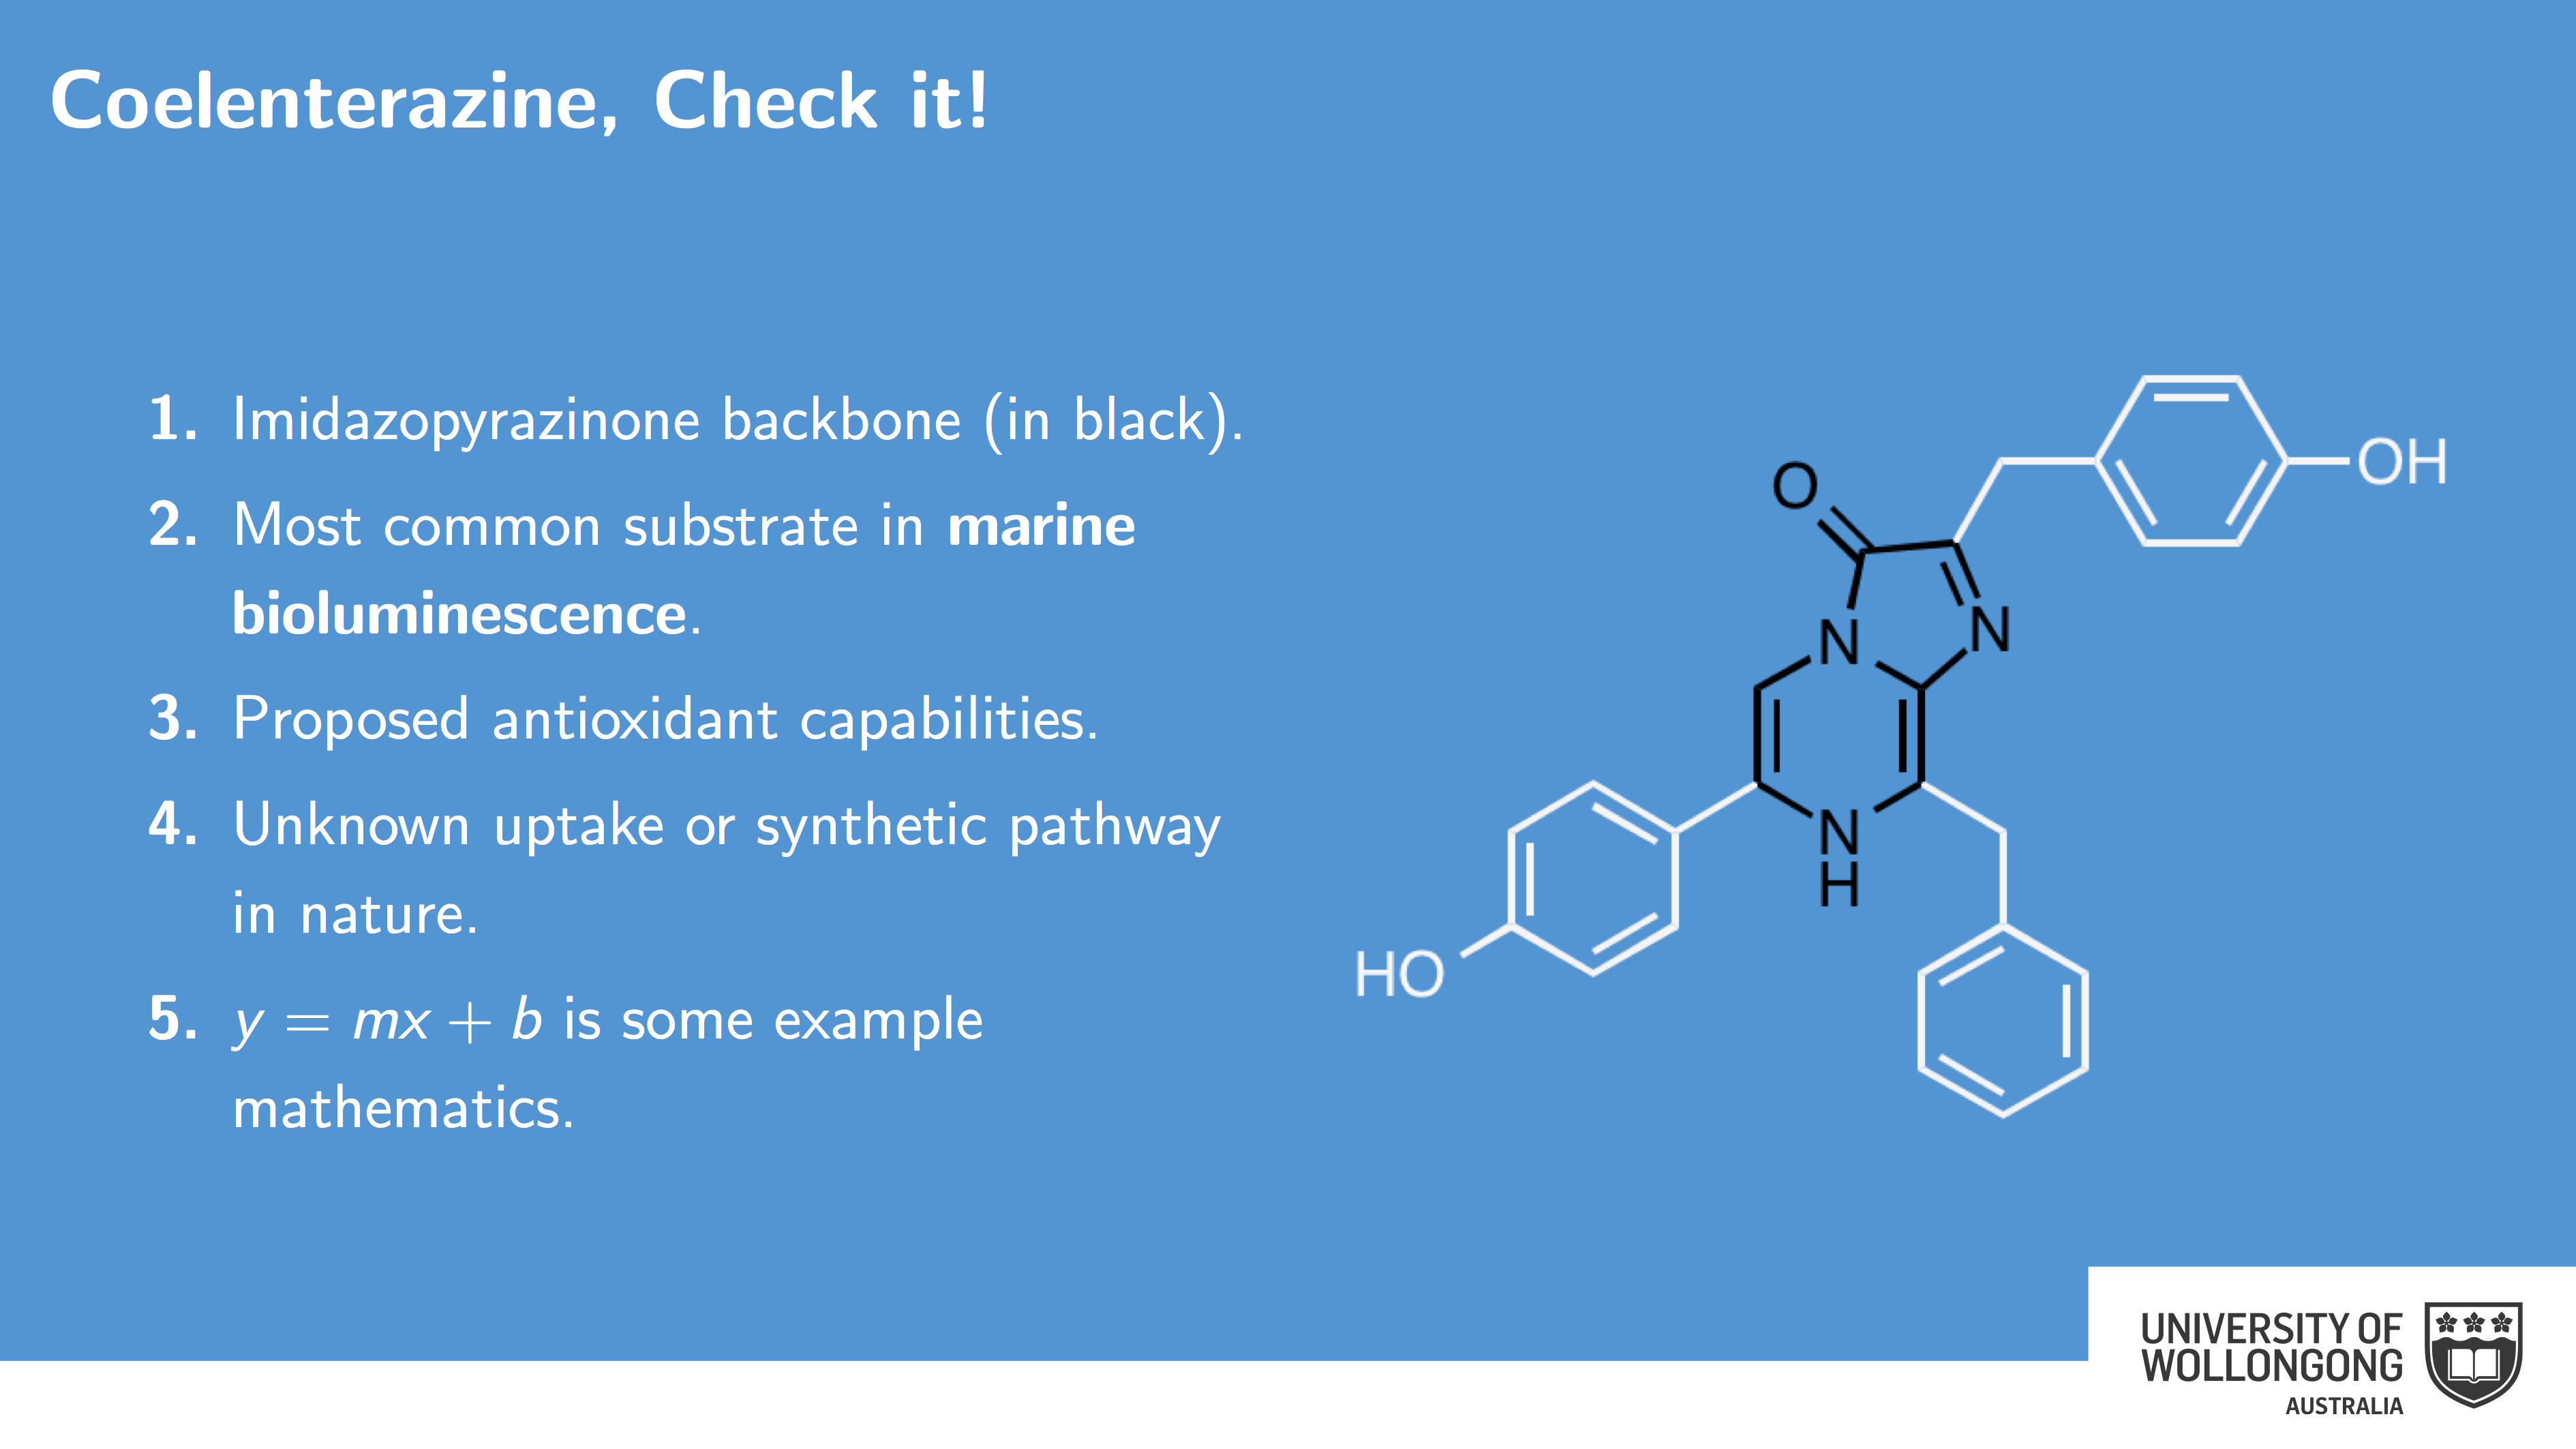
\includegraphics[width=0.5\textwidth]{contentframe_bold.png}}\par

\subsubsection*{\val{boldplain}}% \\[0.5em]
\fbox{
\includegraphics[width=0.5\textwidth]{titleframe_standard.png}}
\fbox{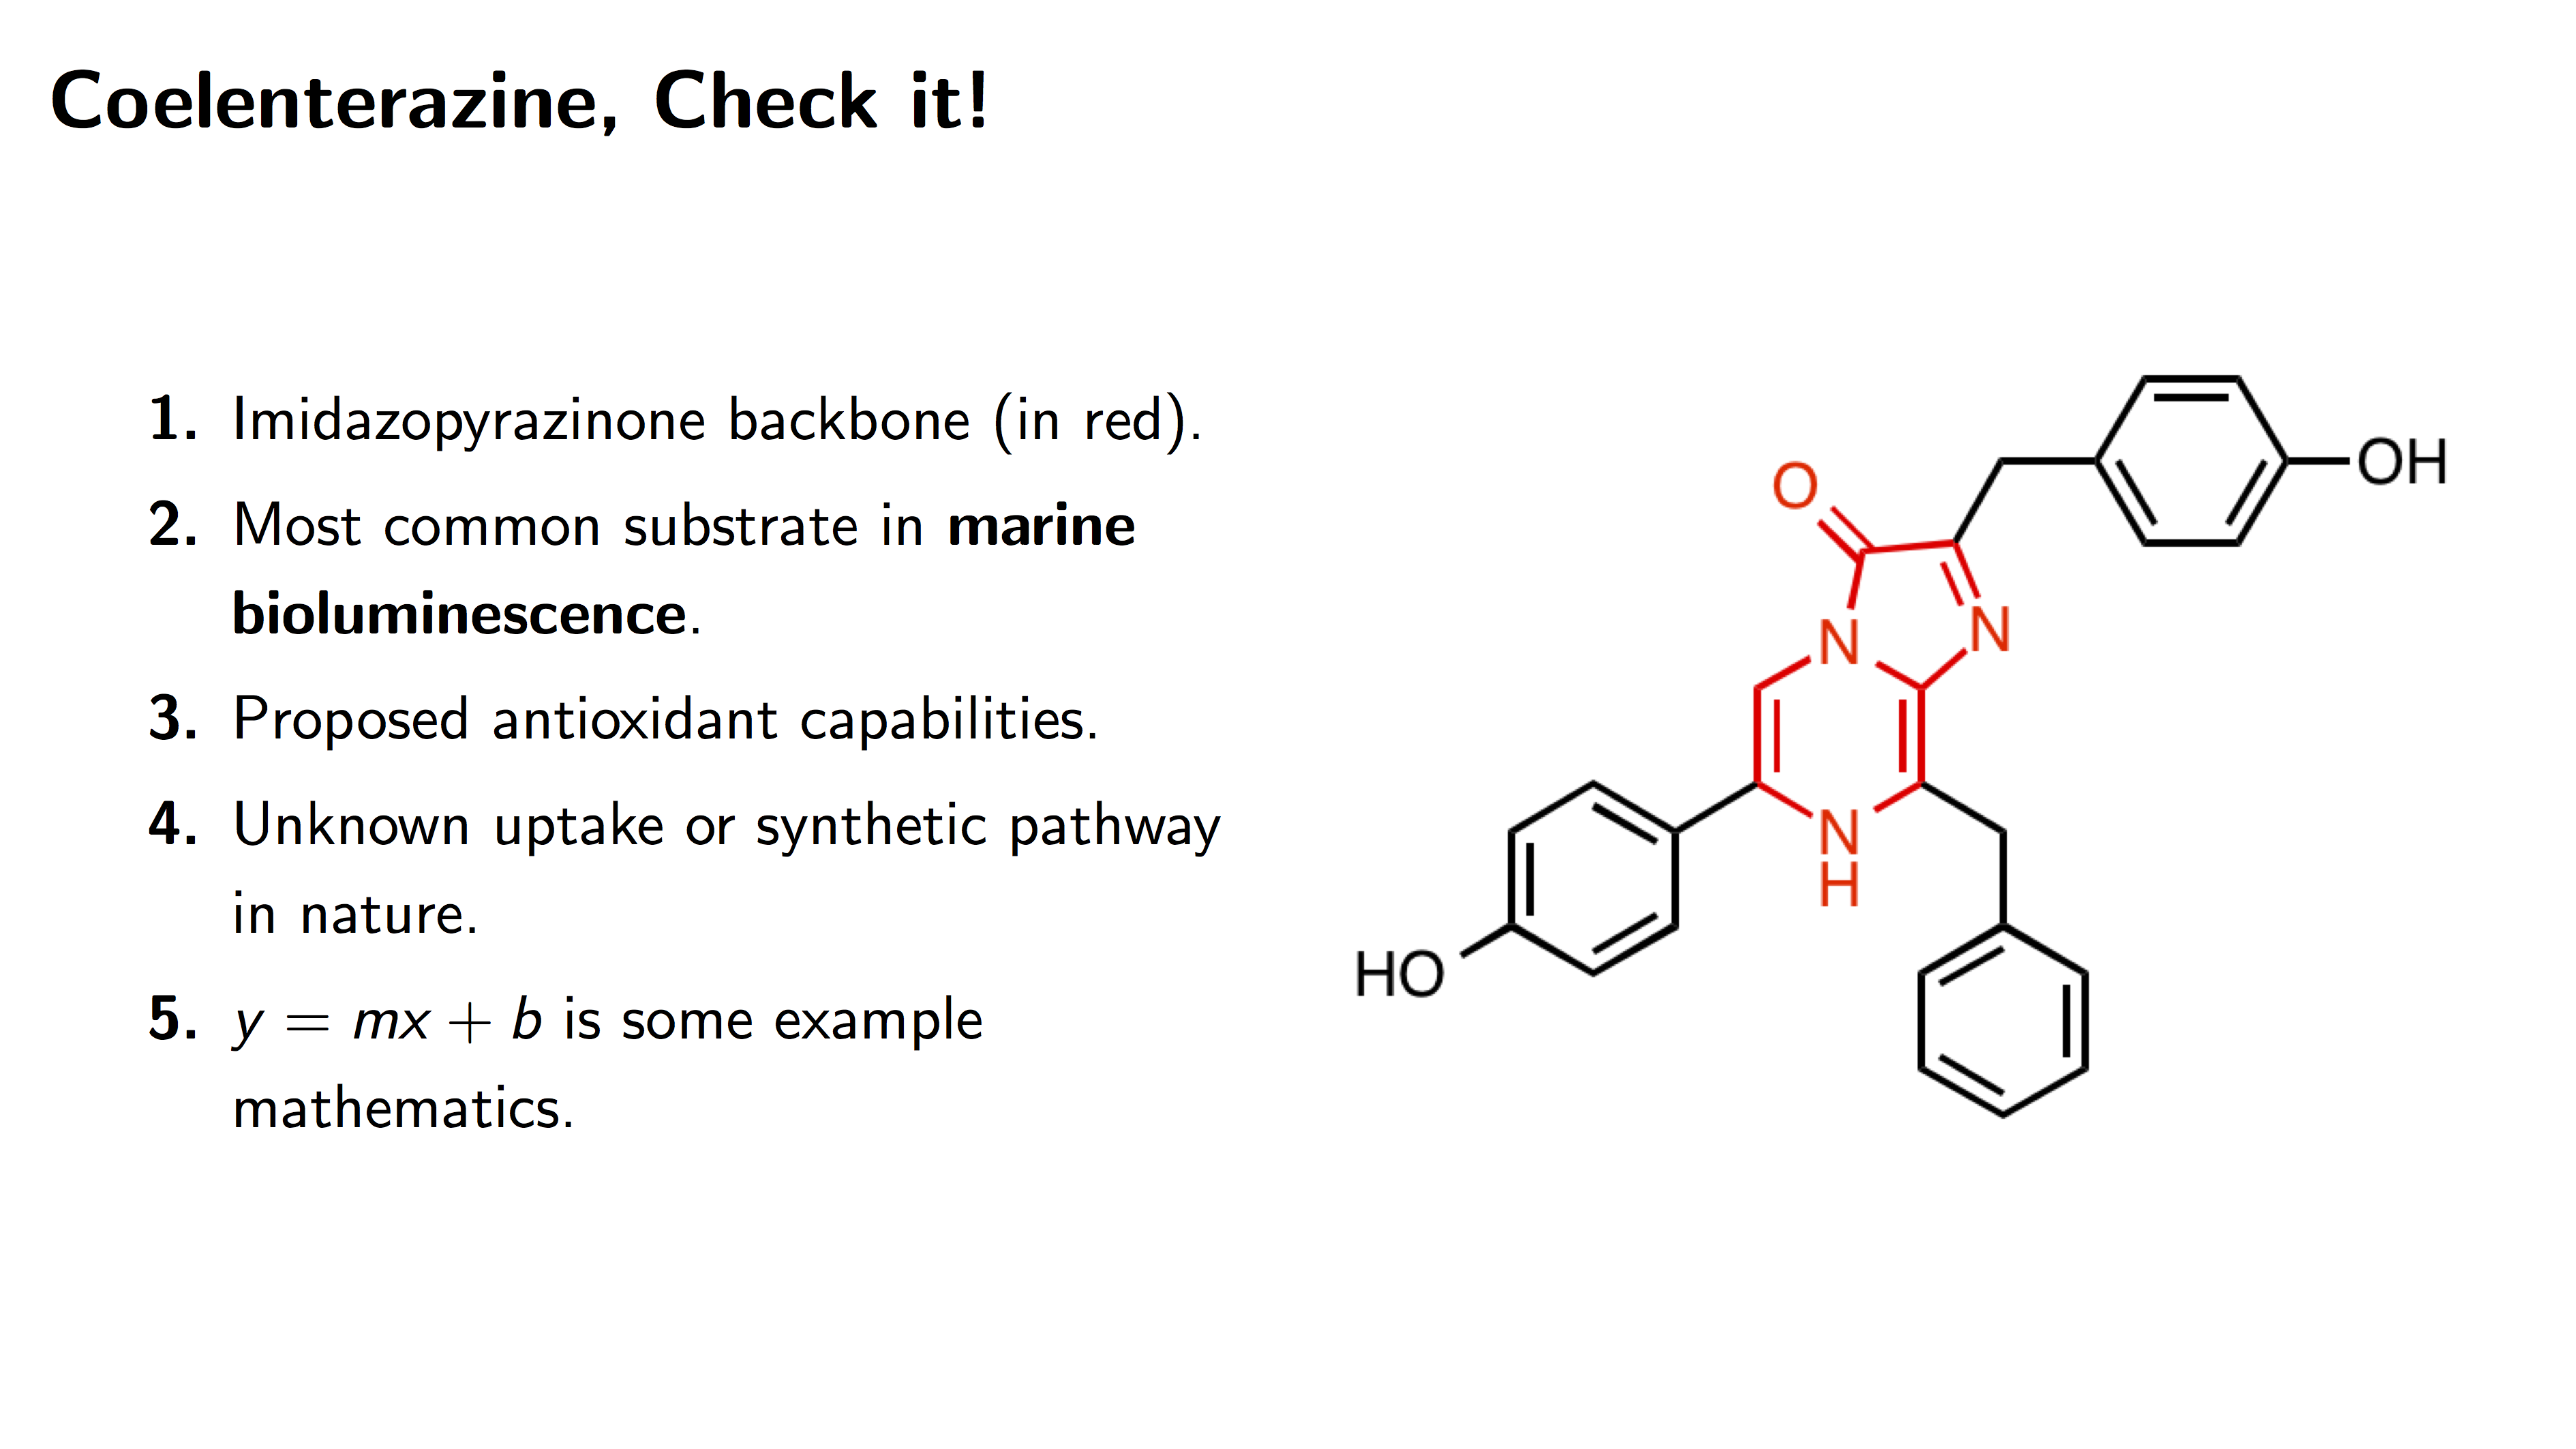
\includegraphics[width=0.5\textwidth]{contentframe_plain.png}}\par

\subsubsection*{\val{eco}}% \\[0.5em]
\fbox{
\includegraphics[width=0.5\textwidth]{titleframe_eco.png}}
\fbox{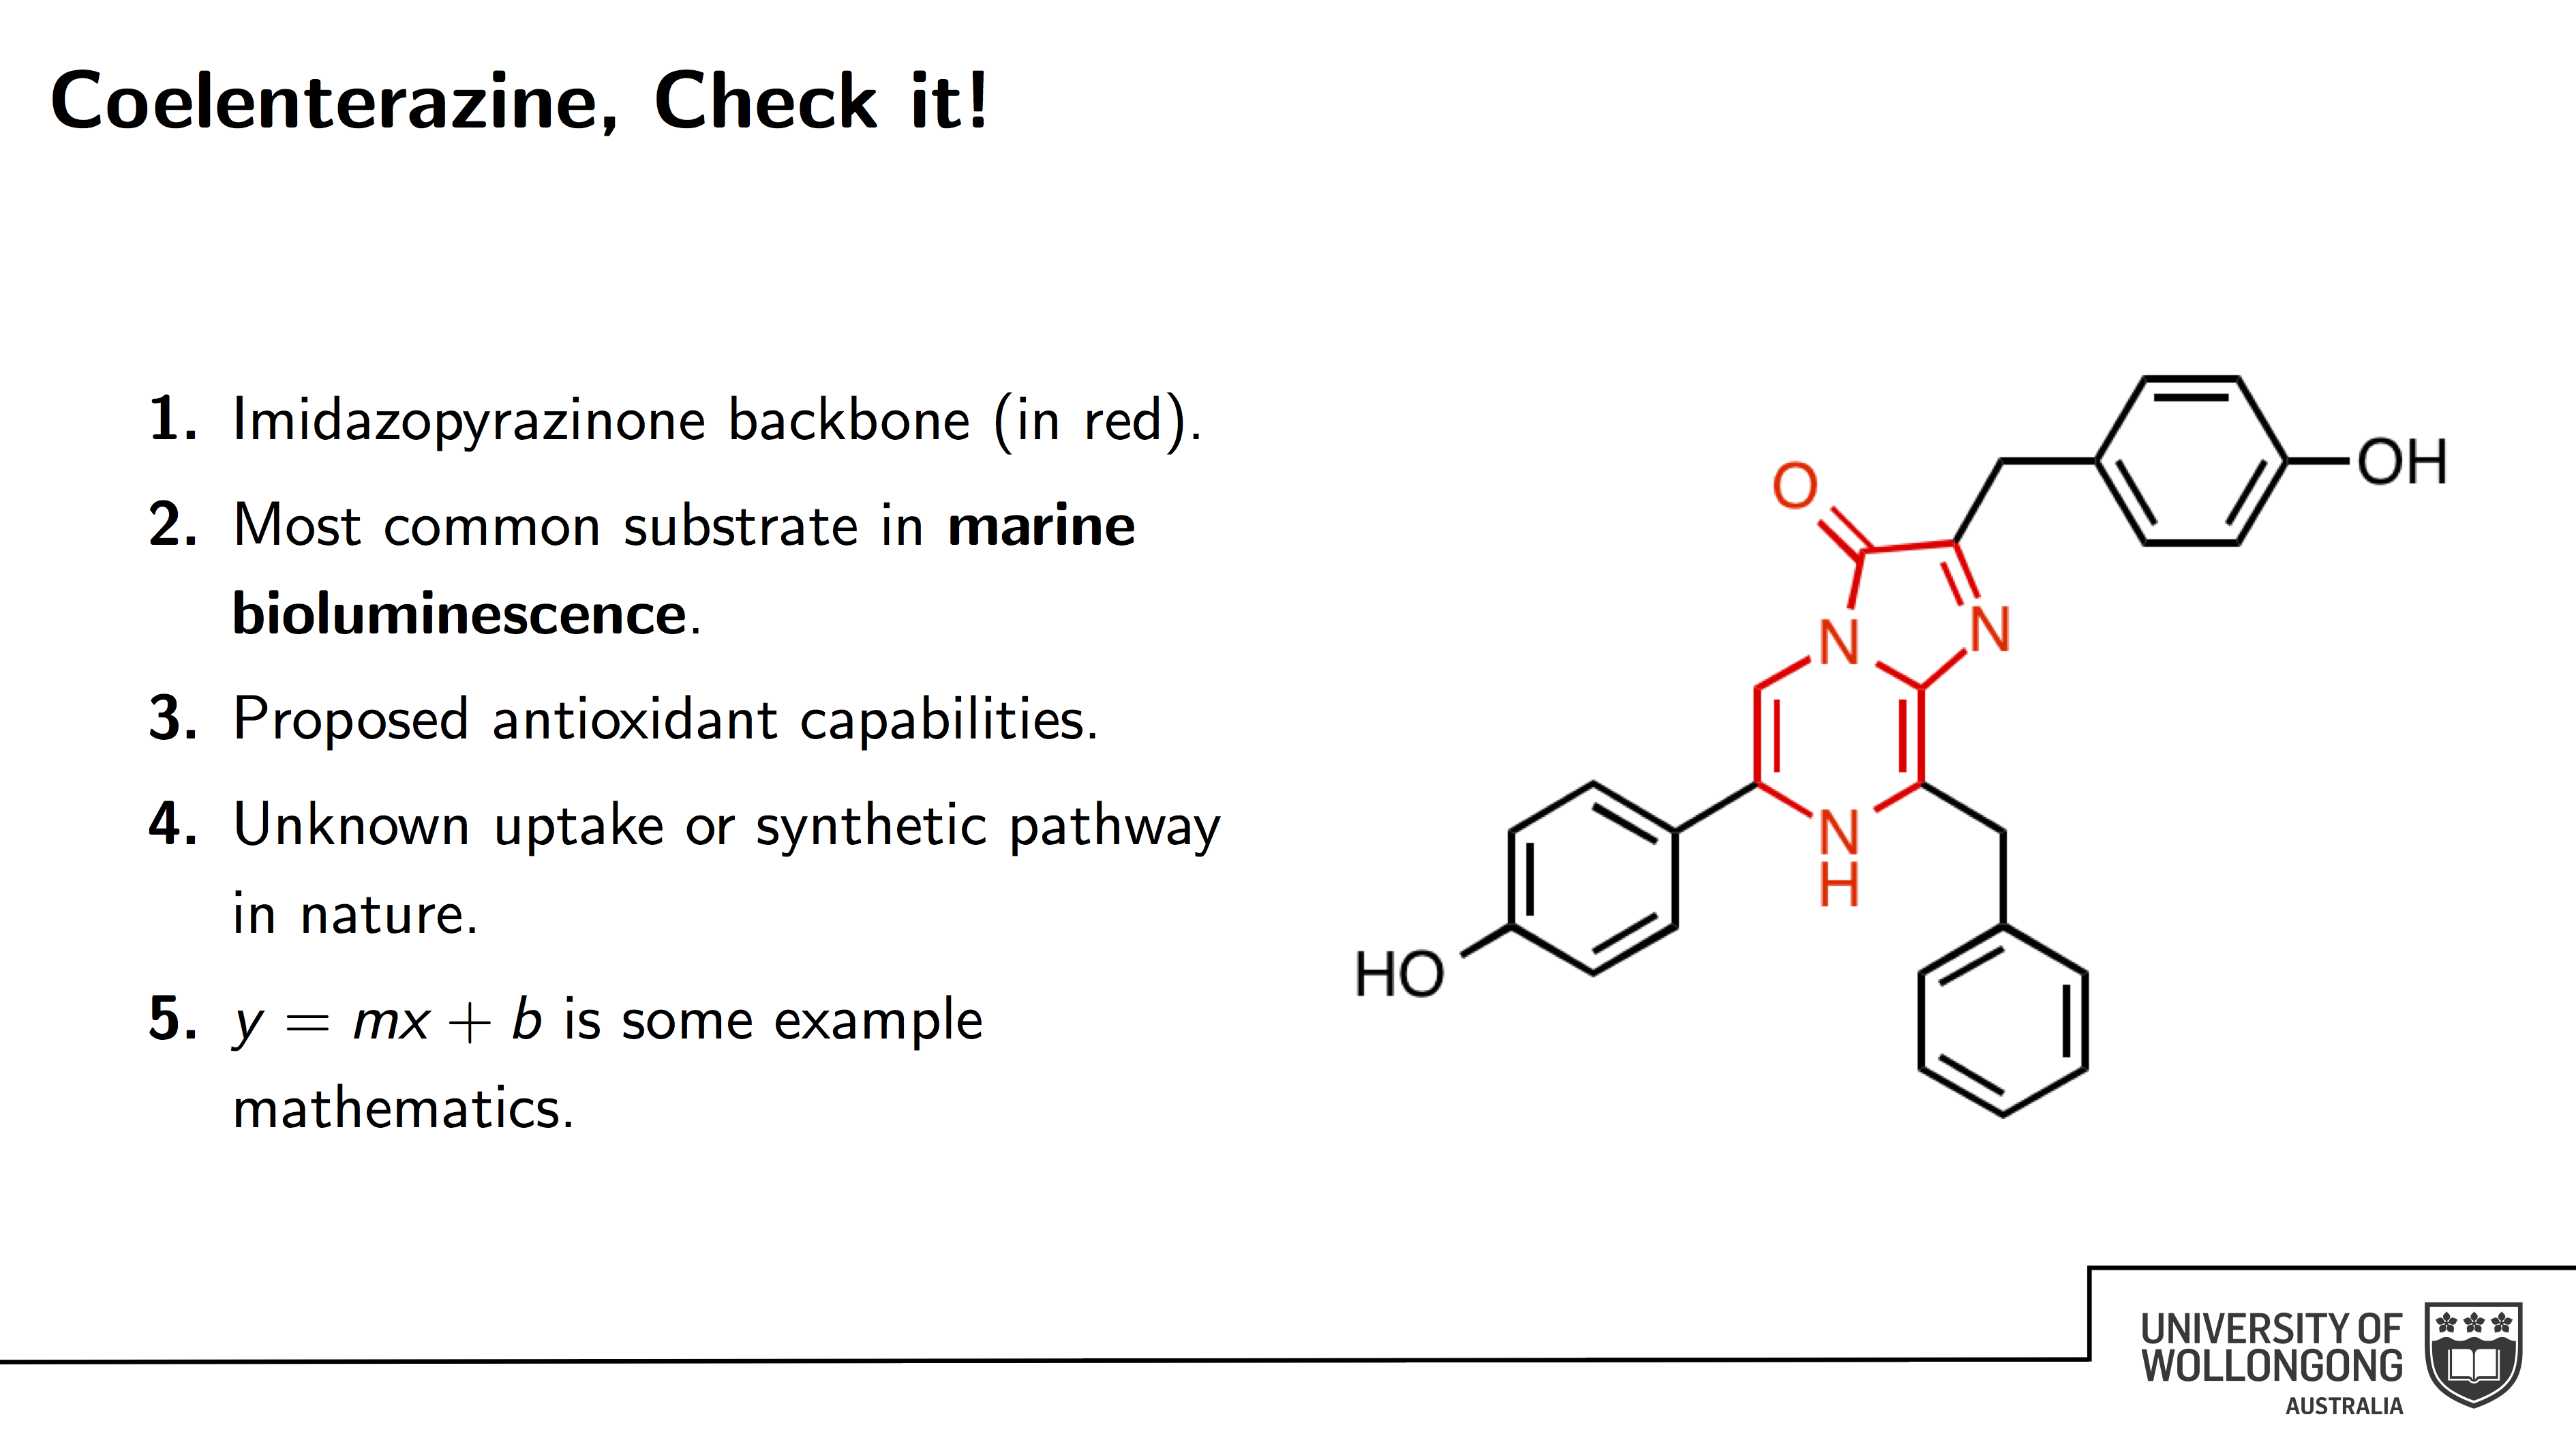
\includegraphics[width=0.5\textwidth]{contentframe_eco.png}}\par

\subsubsection*{\val{ecominimal}}% \\[0.5em]
\fbox{
\includegraphics[width=0.5\textwidth]{titleframe_eco.png}}
\fbox{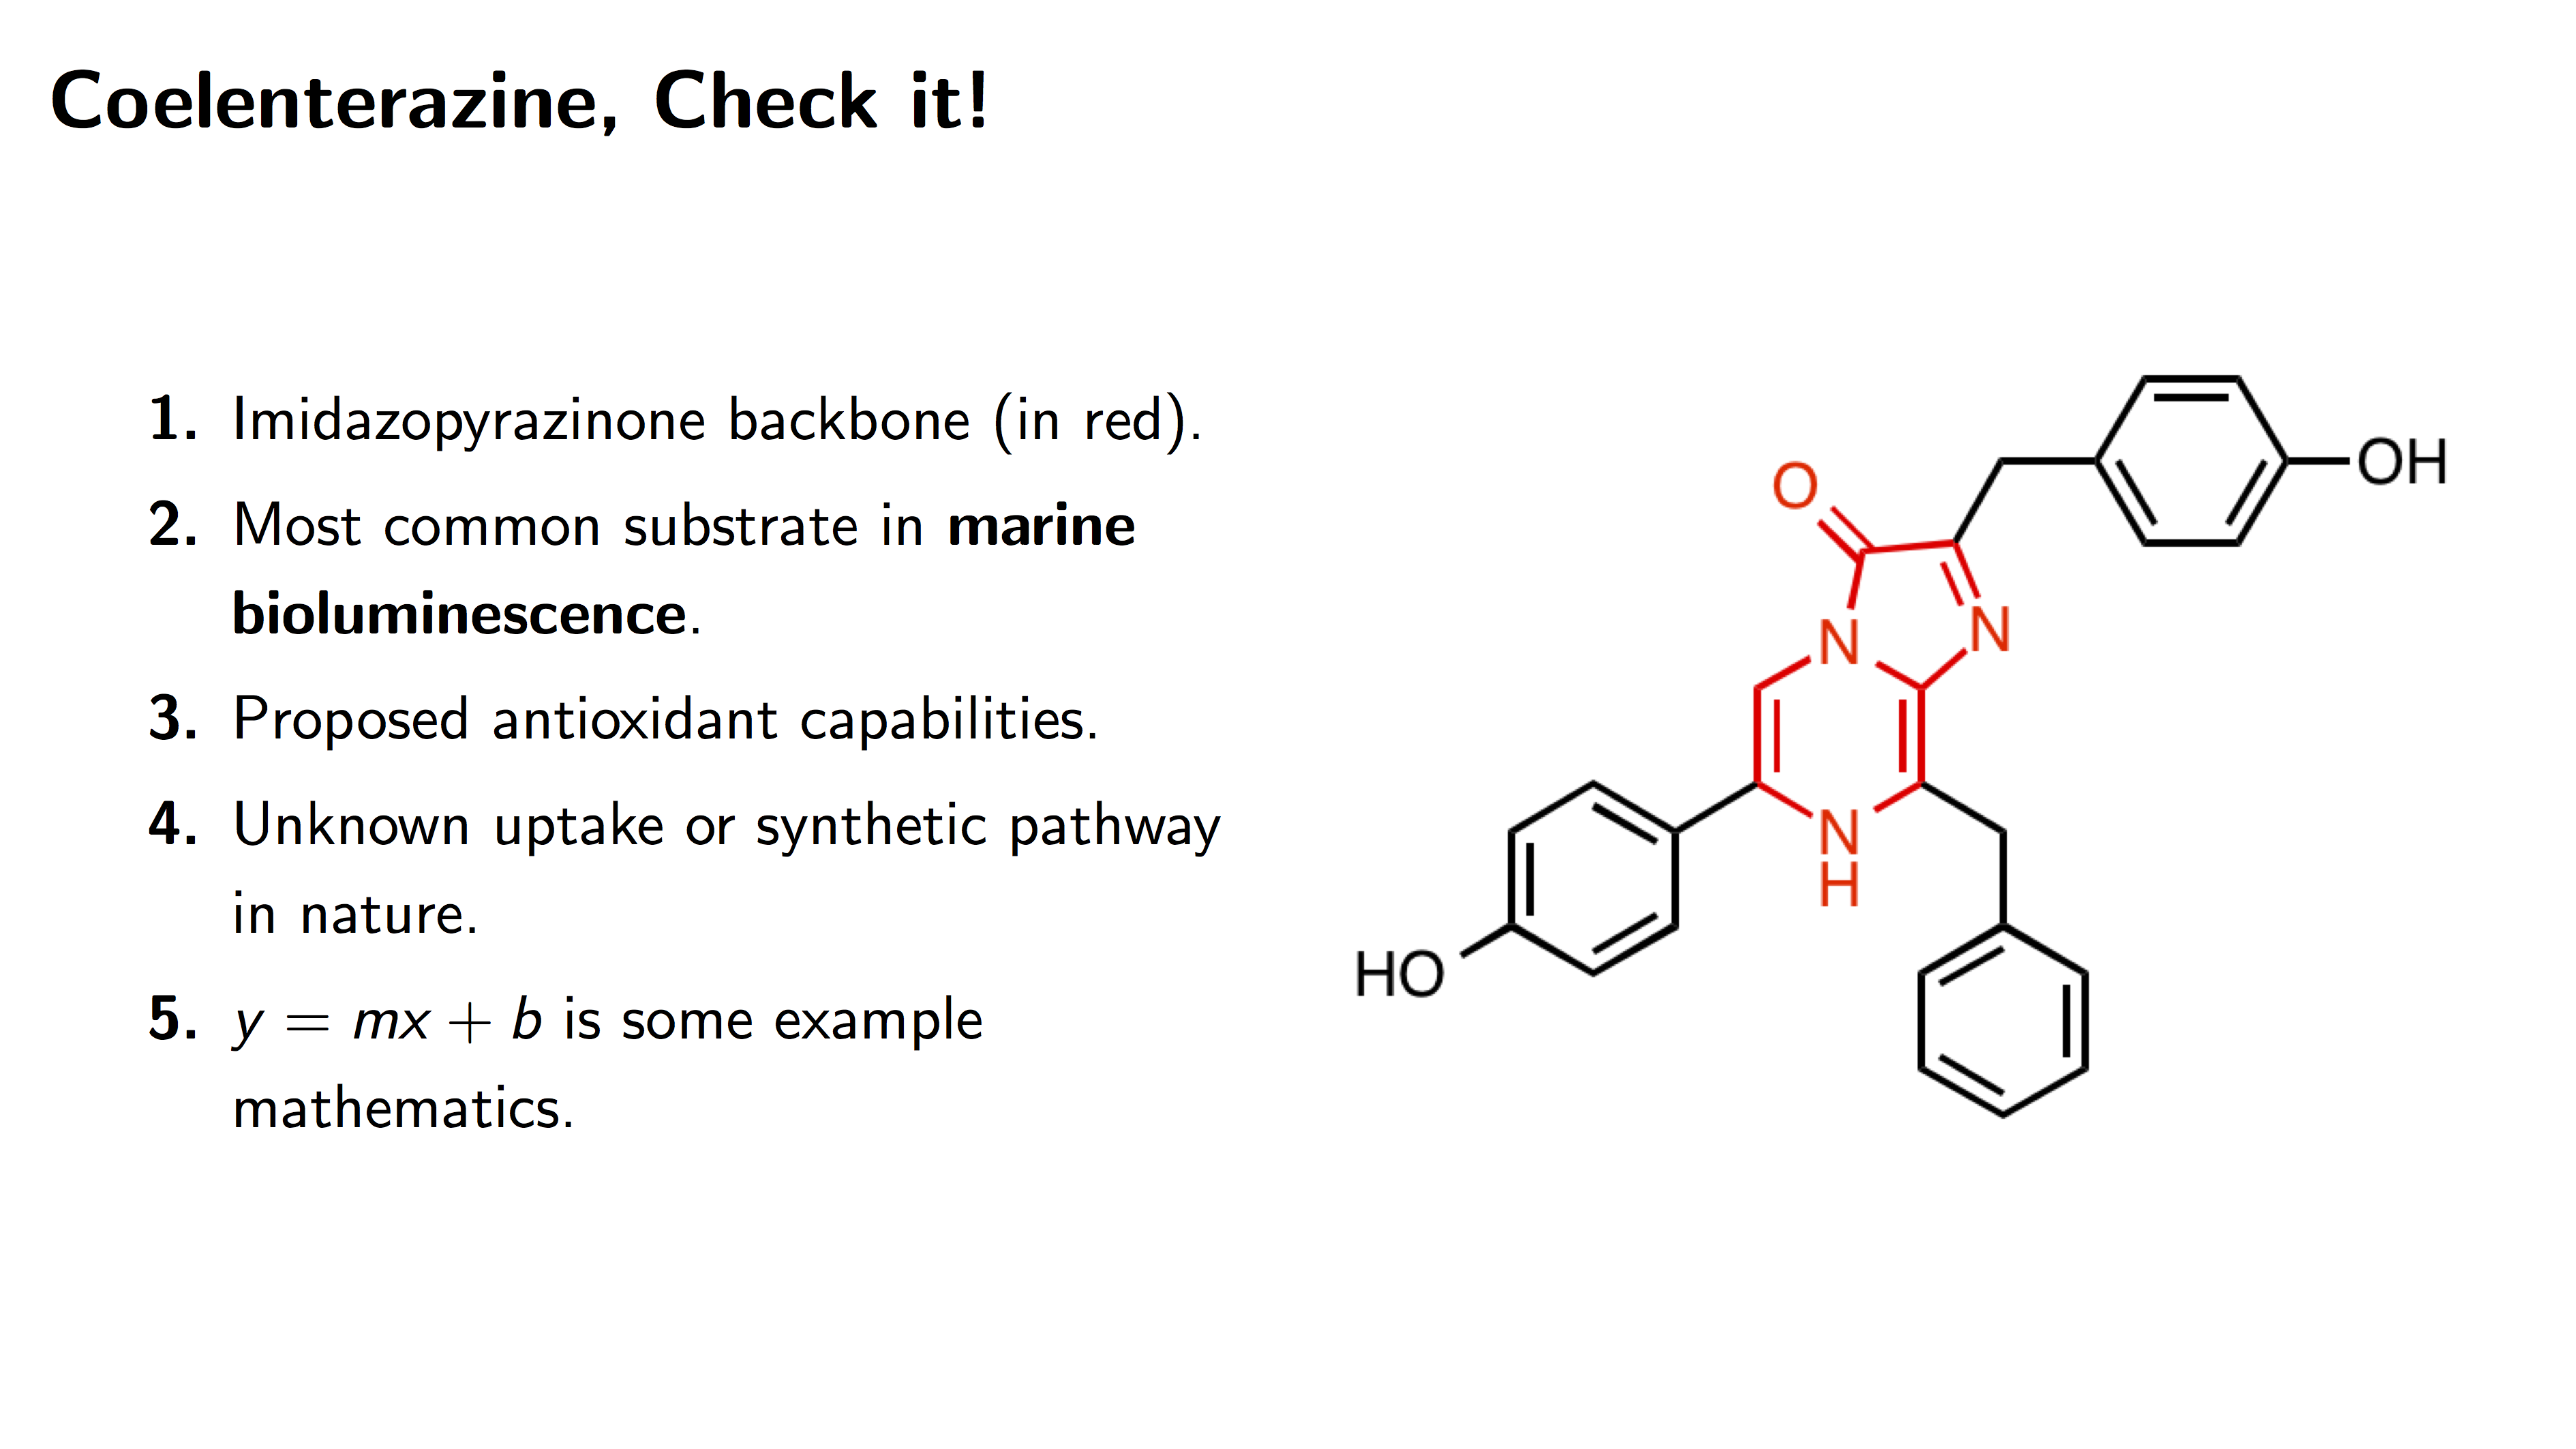
\includegraphics[width=0.5\textwidth]{contentframe_plain.png}}\par

\subsubsection*{\val{plain}}% \\[0.5em]
\fbox{
\includegraphics[width=0.5\textwidth]{titleframe_plain.png}}
\fbox{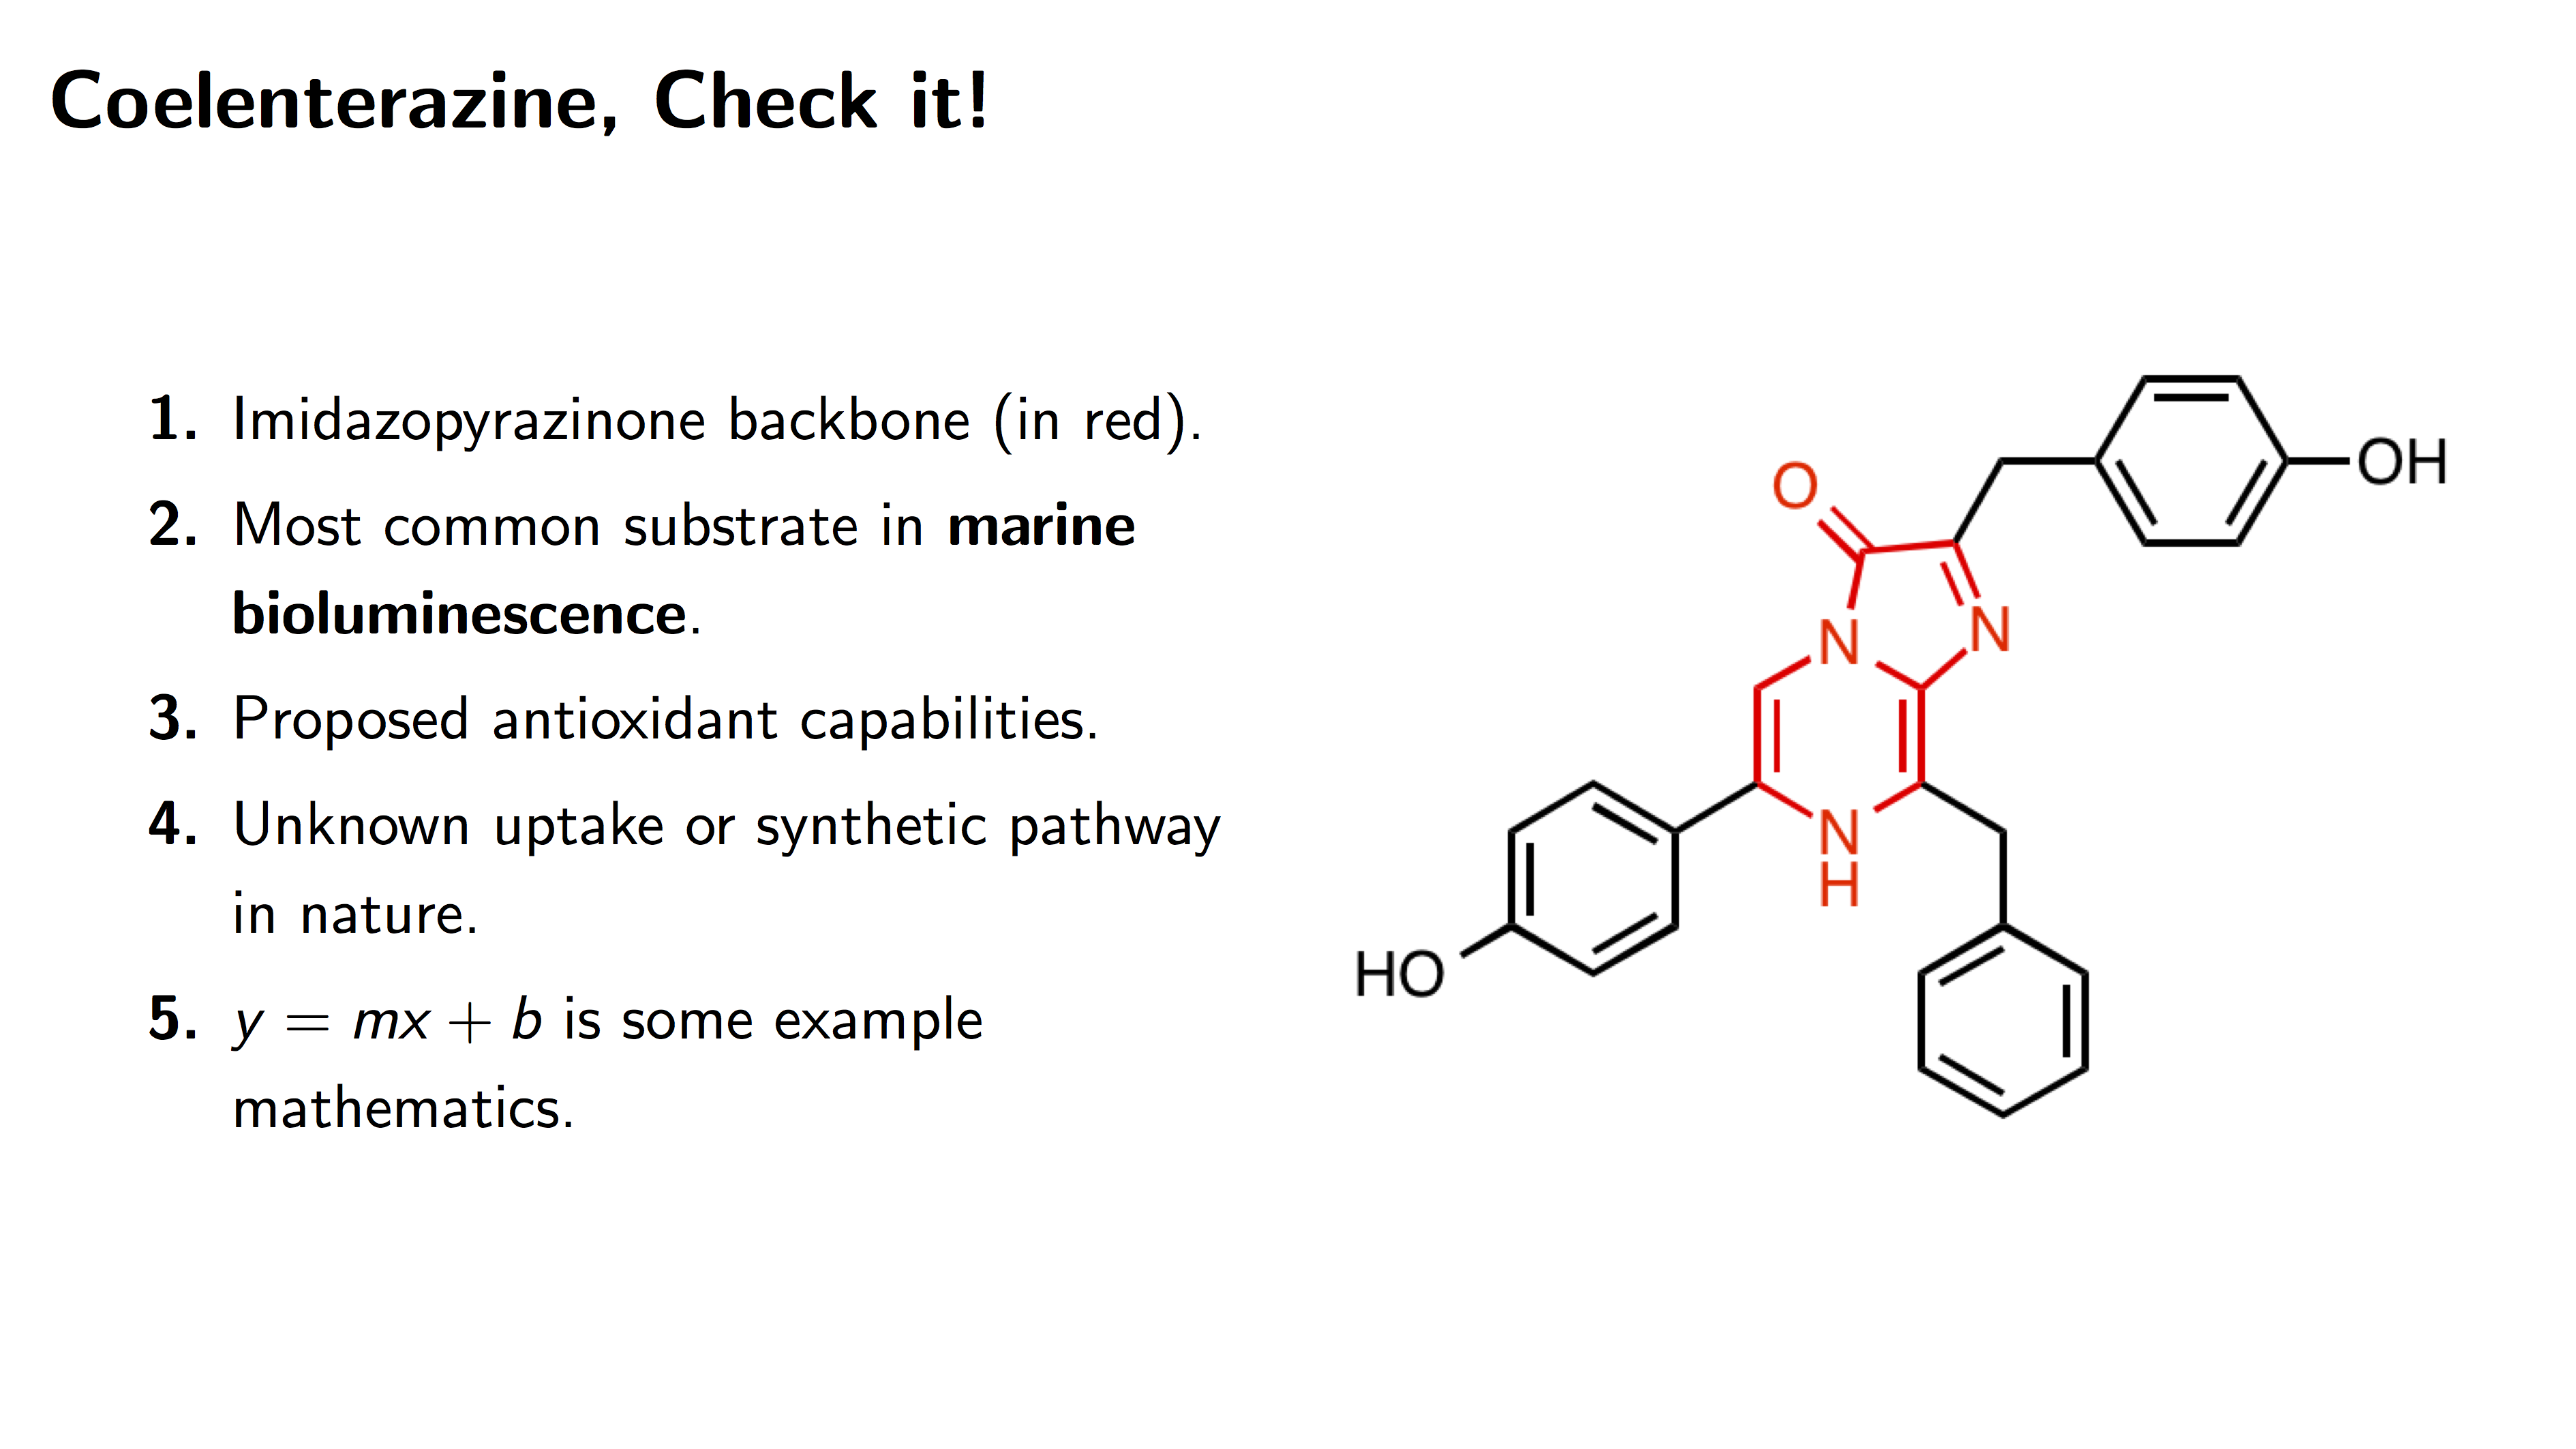
\includegraphics[width=0.5\textwidth]{contentframe_plain.png}}\par


\subsubsection*{\key{themecolor} \textit{or} \key{themecolour}}
Each of the colours outlined in the UOW brand identity guideline are available as colours for the presentation. The key themecolor (or themecolour) sets the colour of the polygons and elements in the UOW theme. These colours can be used in the document to colour any element by calling the colour, for example as an argument to \command{\textbackslash{}color\{UOWred\}}, by prefixing the name of the key with `UOW', e.g. UOWblue.

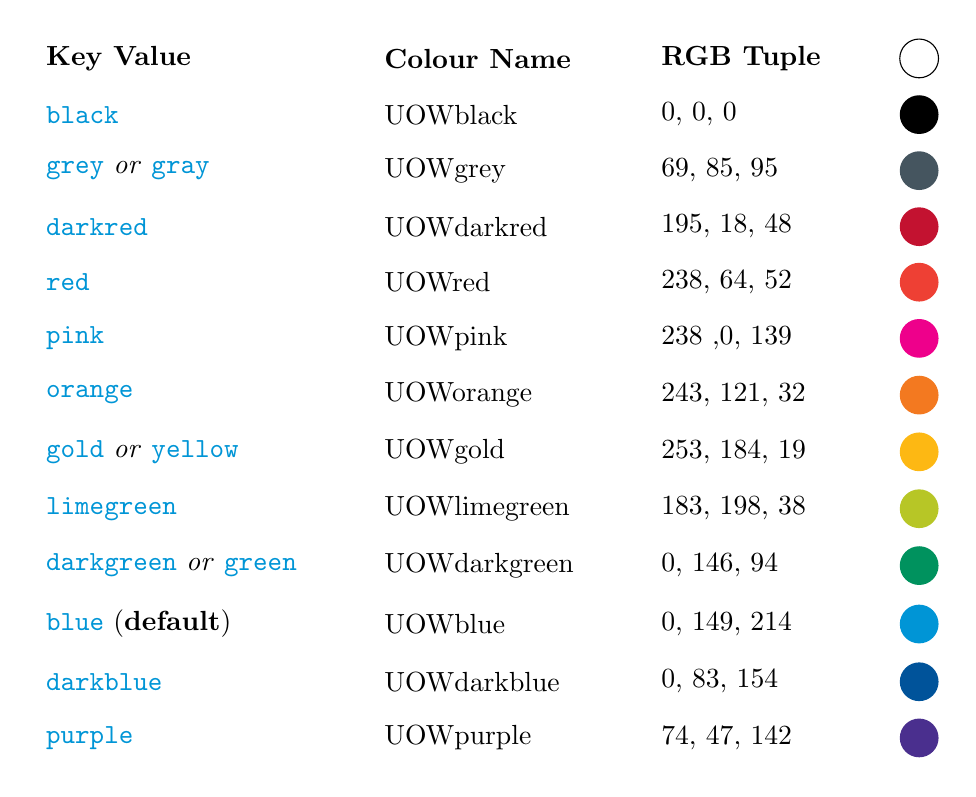
\begin{tikzpicture}[ampersand replacement=\&, every node/.style={anchor=west}] 
\matrix (m) [row sep=0.5em, column sep=2.5em, nodes={align=left}] {%
   \node[align=left] {\textbf{Key Value}}; \& %
   \node[align=left] {\textbf{Colour Name}};   \& %
   \node[align=left] {\textbf{RGB Tuple}};   
   \& \draw [line width=0.4pt, color=UOWblack] (0,0)  circle (0.7em); \\ %
   \node[align=left] {\val{black}};     \& \node[align=left] {UOWblack};     \& \node {0, 0, 0};      %
   \& \fill [line width=1em, color=UOWblack] (0,0)  circle (0.7em); \\
   \node[align=left] {\val{grey} \textit{or} \val{gray}};      \& \node[align=left] {UOWgrey};      \& \node {69, 85, 95};   %
   \& \fill [line width=1em, color=UOWgrey] (0,0)  circle (0.7em); \\
   \node[align=left] {\val{darkred}};   \& \node[align=left] {UOWdarkred};   \& \node {195, 18, 48};  %
   \& \fill [line width=1em, color=UOWdarkred] (0,0)  circle (0.7em); \\
   \node[align=left] {\val{red}};       \& \node[align=left] {UOWred};       \& \node {238, 64, 52};  %
   \& \fill [line width=1em, color=UOWred] (0,0)  circle (0.7em); \\
   \node[align=left] {\val{pink}};      \& \node[align=left] {UOWpink};      \& \node {238 ,0, 139};  %
   \& \fill [line width=1em, color=UOWpink] (0,0)  circle (0.7em); \\
   \node[align=left] {\val{orange}};    \& \node[align=left] {UOWorange};    \& \node {243, 121, 32}; %
   \& \fill [line width=1em, color=UOWorange] (0,0)  circle (0.7em); \\
   \node[align=left] {\val{gold} \textit{or} \val{yellow}};      \& \node[align=left] {UOWgold};      \& \node {253, 184, 19}; %
   \& \fill [line width=1em, color=UOWgold] (0,0)  circle (0.7em); \\
   \node[align=left] {\val{limegreen}}; \& \node[align=left] {UOWlimegreen}; \& \node {183, 198, 38}; %
   \& \fill [line width=1em, color=UOWlimegreen] (0,0)  circle (0.7em); \\
   \node[align=left] {\val{darkgreen} \textit{or} \val{green}}; \& \node[align=left] {UOWdarkgreen}; \& \node {0, 146, 94};   %
   \& \fill [line width=1em, color=UOWdarkgreen] (0,0)  circle (0.7em); \\
   \node[align=left] {\val{blue} (\textbf{default})};      \& \node[align=left] {UOWblue};      \& \node {0, 149, 214};  %
   \& \fill [line width=1em, color=UOWblue] (0,0)  circle (0.7em); \\
   \node[align=left] {\val{darkblue}};  \& \node[align=left] {UOWdarkblue};  \& \node {0, 83, 154};   %
   \& \fill [line width=1em, color=UOWdarkblue] (0,0)  circle (0.7em); \\
   \node[align=left] {\val{purple}};    \& \node[align=left] {UOWpurple};    \& \node {74, 47, 142};  %
   \& \fill [line width=1em, color=UOWpurple] (0,0)  circle (0.7em); \\
};
\end{tikzpicture}


\subsubsection*{\key{framnetitlenumbering}}
You can turn on numbering of the slides with this key. The numbers are placed in the bottom right corner of the slides. It does not make much sense to use this option with the \val{standard}, \val{bold}, \val{minimaltitle} and \val{eco} layouts. I may patch this at a later date to place the slide numbers in a different location in these cases, such as the top right corner. For now it is up to the operators discretion to use this option appropriately.

\subsubsection*{\val{counter}}
A plain arabic numeral in the bottom right corner of the slide to show the slide number.

\subsubsection*{\val{fraction}}
A fraction of the page number and the total number of slides separated by a solidus, for example: 3/10.

\subsubsection*{\val{none} default}
No page numbering. This is the default option.


\subsubsection*{\key{titlepage}}
This turns the different background for the first slide on or off depending weather or not you're going to use a title page slide. The options are \val{true}, \val{false} and \val{none}. Each option is fairly self explanatory.


\section{Legal}
This work may be distributed and/or modified under the conditions of the LaTeX Project Public License version 1.3c which can be found \href{http://www.latex-project.org/lppl/lppl-1-3c.txt}{here}\footnote{\url{http://www.latex-project.org/lppl/lppl-1-3c.txt}}.

The crest and associated branding of the University of Wollongong is copyright and the property of the University of Wollongong. As the core identifier of the university its use is governed by the university's brand and visual identity guidelines which can be found \href{http://www.uow.edu.au/about/brand/uowlogo/index.html}{online}\footnote{\url{http://www.uow.edu.au/about/brand/uowlogo/index.html}}

This work is copyright (CC BY-NC-SA 4.0 International Licence) 2015 by T. M. Griffiths under the creative commons licence (attribution, non-commercial, share alike). More information can be found \href{http://creativecommons.org/licenses/by-nc-sa/4.0/}{here}\footnote{\url{http://creativecommons.org/licenses/by-nc-sa/4.0/}}. Inspiration for parts of this theme (where design decision had to be made) and guidance on the implementation of the pgfkeys were taken from the \href{https:/github.com/matze/mtheme}{metropolis theme}\footnote{\url{https:/github.com/matze/mtheme}} by Matthias Vogelgesang \textit{et al}., of which the author is a contributor. 

\vspace{1em}\begin{center}\ccbysa\end{center}


\section{Change Log}
If you spot any errors or bugs, or alternately you have any requests for an addition let me know.
\subsection*{Version 1.0, 2015–07–23, tmgriffiths}
It's day dot. Nothing to added or removed. It just is.

\end{document}